\paragraph{Sơ đồ tuần tự luồng Theo dõi báo cáo Pháp Điển Pipeline}

Luồng nghiệp vụ này mô tả
quy trình Quản trị viên (Admin) theo dõi, kiểm tra báo cáo thống kê của luồng xử lý dữ liệu Pháp Điển Việt Nam tự động (Pháp Điển Pipeline) thông qua giao diện Bảng điều khiển (Admin Dashboard).

\begin{figure}[H]
\centering
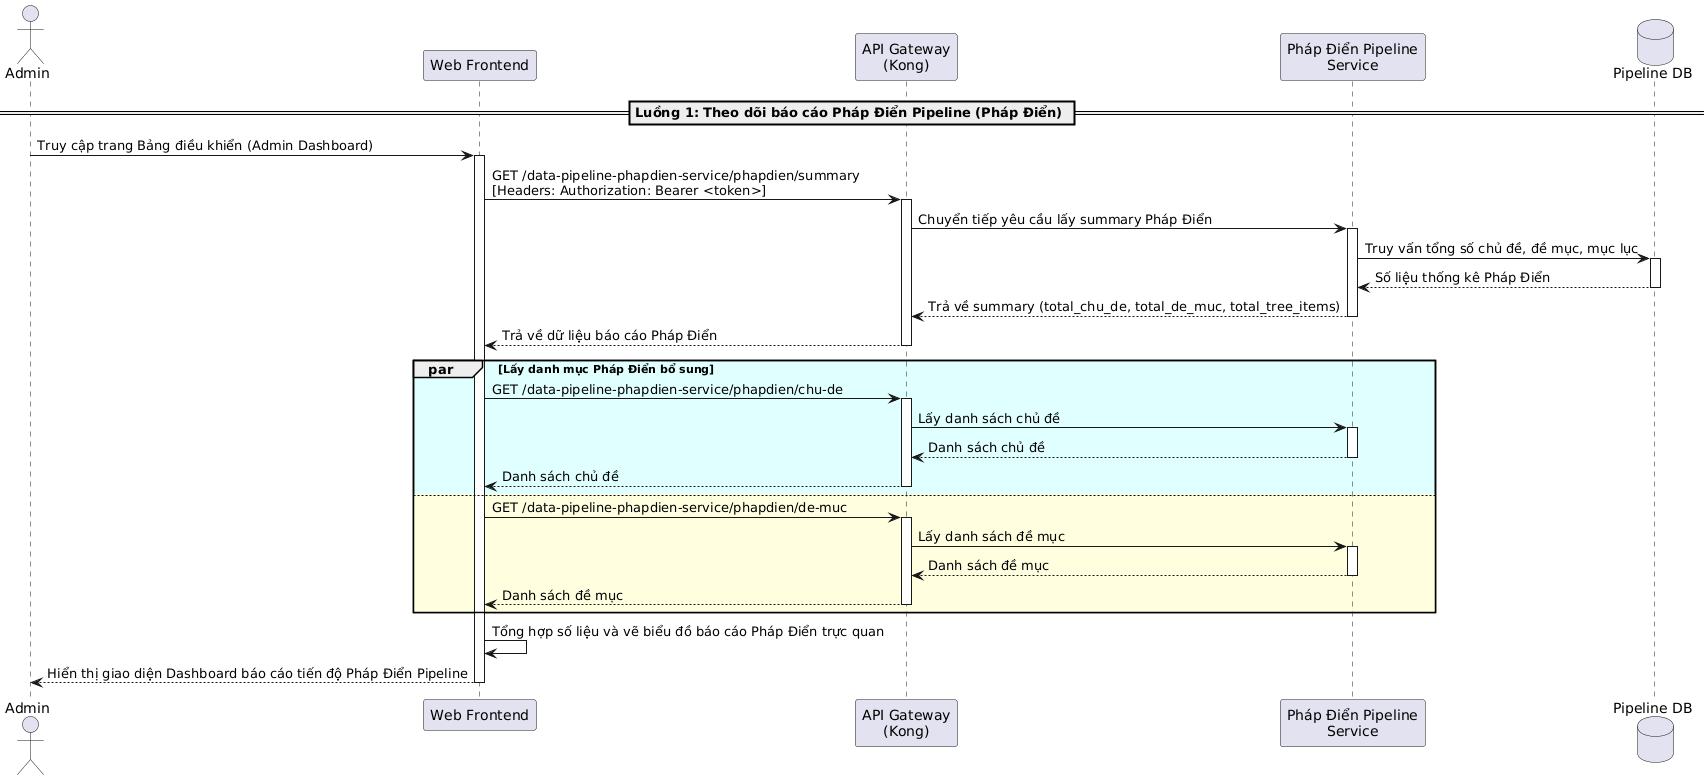
\includegraphics[scale = 0.2]{contents/Sequence/UML-Sequence-AdminPhapDienPipelineReport.png}
\caption{Sơ đồ tuần tự luồng Theo dõi báo cáo Pháp Điển Pipeline}
\end{figure}

\subparagraph{Các thành phần tham gia}

\begin{table}[H]
\centering
\renewcommand{\arraystretch}{1.3}

\begin{tabular}{|l|l|p{5cm}|}
\hline
\textbf{Thành phần} & \textbf{Phân loại} & \textbf{Vai trò trong hệ thống} \\ \hline
Admin & Actor & Quản trị viên truy cập bảng điều khiển để giám sát hệ thống. \\ \hline
Web Frontend & Component & Giao diện web Next.js. \\ \hline %%%% Component & Giao diện Admin Dashboard biểu diễn số liệu dưới dạng đồ thị và bảng số liệu. \\ \hline
API Gateway (Kong) & Component & Cổng API chuyển tiếp các yêu cầu API. \\ \hline %%%% Component & Định tuyến yêu cầu thống kê tới Pháp Điển Pipeline Service và kiểm tra quyền Admin. \\ \hline
Pháp Điển Pipeline Service & Microservice & Dịch vụ xử lý dữ liệu Pháp Điển, cung cấp số liệu tổng hợp về chủ đề, đề mục. \\ \hline
Pipeline Database & Database & CSDL lưu trữ kết quả thống kê cấu trúc cây Pháp Điển. \\ \hline
\end{tabular}
\caption{Các thành phần tham gia luồng Theo dõi báo cáo Pháp Điển Pipeline}
\end{table}

\subparagraph{Mô tả tổng quan}

\begin{itemize}
\item \textbf{Yêu cầu xem báo cáo:}
Quản trị viên truy cập màn hình báo cáo. Giao diện gửi yêu cầu lấy số liệu thống kê về tiến trình xử lý dữ liệu pháp điển qua cổng API.
\item \textbf{Kiểm tra và định tuyến:}
Cổng API chuyển tiếp yêu cầu đến dịch vụ xử lý dữ liệu pháp điển. % Cổng API xác thực thông tin đăng nhập của quản trị viên và chuyển tiếp yêu cầu đến dịch vụ xử lý dữ liệu pháp điển.
\item \textbf{Thống kê dữ liệu:}
Dịch vụ xử lý dữ liệu pháp điển truy vấn CSDL thống kê để lấy tổng số chủ đề, tổng số đề mục và tổng số nút thư mục trong hệ thống pháp điển, sau đó phản hồi số liệu tổng hợp về giao diện.
\item \textbf{Lấy danh mục bổ sung:}
Giao diện gửi thêm yêu cầu lấy chi tiết danh mục chủ đề và đề mục để hiển thị thông tin trực quan.
\item \textbf{Biểu diễn thông tin:}
Giao diện nhận dữ liệu, tính toán tiến độ hoàn thành và vẽ biểu đồ trực quan giúp quản trị viên dễ dàng theo dõi tiến trình.
\end{itemize}
